\subsection{Independent component clustering and grand-average ERSP}
We used the above result as a region of interest (ROI) seed for the repetitive cluster optimization approach. This resulted in a cluster solution containing an optimal central-parietal cluster with a centroid location around X = -2,Y = -37, Z = 46 (MNI), a mean residual variance of 5\%, containing 17 of 19 participants and 21 independent components. Providing an overview for the cluster of interest, the grand-average time-frequency characteristics are a useful guide for the following single-trial investigation. In the grand scheme, the task elicited increased theta-band activity following the appearance, or spawn, of the target to be selected ($t_{16} = 4.02, P = 0$ at -300 ms and 5 Hz). A similar theta-band signature, albeit to a lesser extent, was observed following spatio-temporal asynchronous object selection indicated by color change and vibration in the vibrotactile trials ($t_{16} = 2.16, P = 0.02$ at 270 ms and 4.5 Hz). Further, theta-band activity exceeded baseline activity during the randomized interval leading up to the object spawn. Significant alpha- and beta-band power decrease was observed during the trial hand movement phase ($t_{16} = -3.37, P = 0$ at 0 ms and 12 Hz; $t_{16} = -5.87, P = 0$ at 0 ms and 21 Hz) as well as leading up to the object spawn, predominantly in the beta-band ($t_{16} = -3.85, P = 0$ at -2200 ms and 21 Hz). Beta-band power increase outlasted alpha-band power increase after ~1s following asynchronous object selection ($t_{16} = -4.22, P = 0.003$ at 1100 ms and 21 Hz), \ref{grand_average_ersp} B.
\begin{figure}[t]
  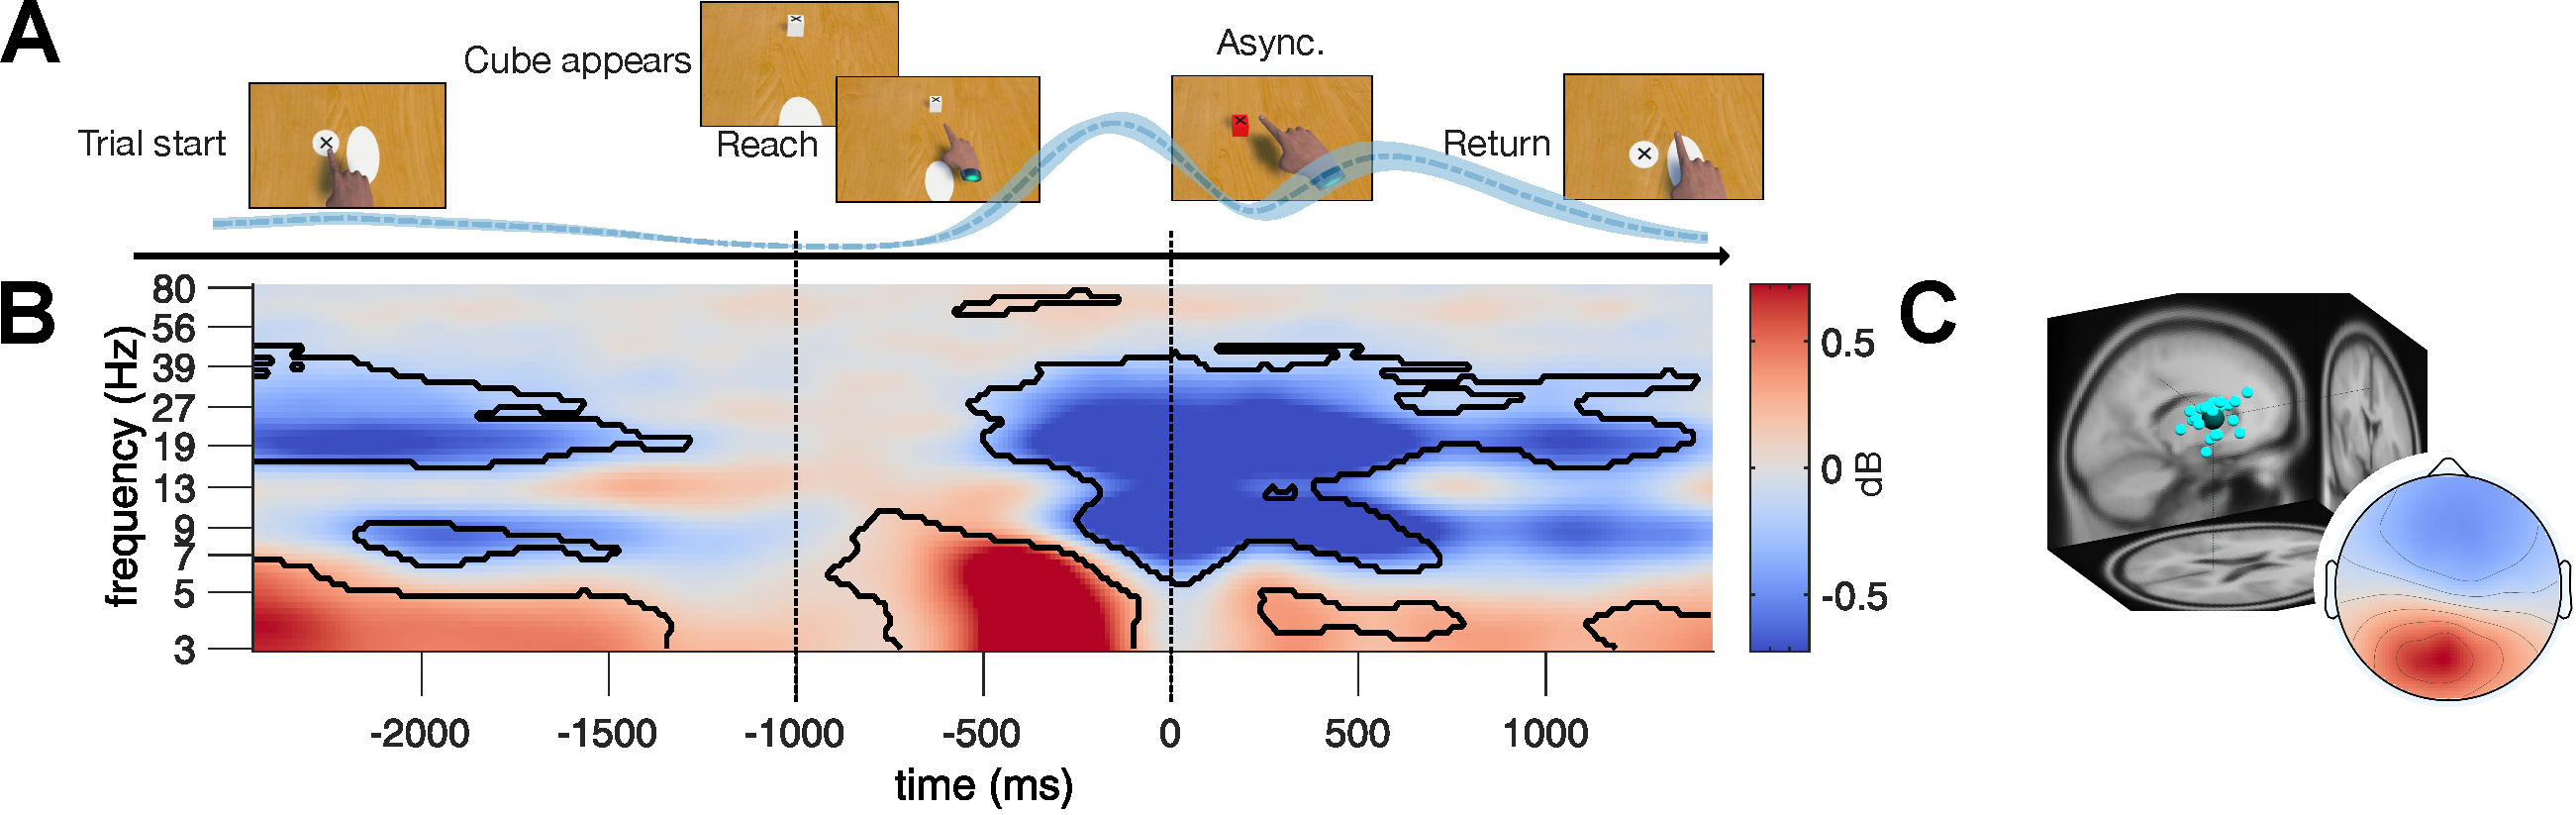
\includegraphics[width=\textwidth]{figures/fig3_context_grand-average_short.pdf}
  \caption{\textbf{A} Task and velocity profile of asynchronous trials. \textbf{B} Grand-average event-related spectral perturbations, that is changes in logarithmic scale over a divisive baseline. Black lines enclose areas of significant regions containing at least 50 pixels below P = .05 calculated using permutation t-tests. For visualization, time-frequency maps were smoothed with a Gaussian (width = 1.5). \textbf{C} Dipole of clustered independent components and the cluster mean scalp map of the optimal cluster seeded with LDA results.}
  \label{grand_average_ersp}
\end{figure}

%at X = 21,Y = -56, Z = 31 (MNI), mean residual variance of 7\%, containing 17 out of 19 participants and 18 independent components. Optimizing for the central-parietal ROI resulted in a cluster solution with an optimal cluster located around X = -2,Y = -37, Z = 46 (MNI) with a mean residual variance of 5\%, containing 17 of 19 participants and 21 independent components. There was no overlapping independent component present in both clusters. 
%In the right occipito-parietal cluster, a high alpha-band (12-18 Hz) power increase pre- and succeeded the hand movement phase, see \ref{grand_average_ersp} D and \ref{velocity} C top to bottom. 